\documentclass[11pt]{report}

\usepackage{hyperref}
\usepackage{graphicx} %Package f�r Grafiken
\usepackage{subfig} % Package f�r mehrere Grafiken nebeneinander
\usepackage{amsmath}
\DeclareMathOperator{\atantwo}{atan2}

\begin{document}
\chapter{Date Cleaning and Preparation}

\section{New York Inspection Data}

The main dataset for our project is retrieved from the \href{https://data.ny.gov/Economic-Development/Retail-Food-Store-Inspections-Current-Ratings/d6dy-3h7r}{official site of the State of New York}. It contains a total of 28'300 A to C ratings from of food store inspections. When we downloaded the data on the XXX it has been the version of June 26, 2019 with observations from March 2018 to March 2019.\\
\\
--> here Kaspar remove duplicate values
\\
We will predict the food store inspection ratings from this dataset with different covariates whose derivation is outlined in the following sections.

\section{Chain Information}

\section{Spatial Data}

Some of the predictors rely on geolocation data. The cleaned inspection dataset contain spatial information in form of latitude and longitude data for most of the observations. The latitude and longitude information, however, is embedded in a larger address string. We create a function to extract the location data in two new columns. A check for \texttt{NA} values reveals that 748 values missing location information. The exact address is available for all shops though. Therefore, we combine, street, city and ZIP code to a single string that can be used with the Google Maps API\footnote{In essence, the Google Maps API is a free service offered by Google. It requires only a one-time registration with a valid email address. Afterwards, it generates an API Key that must be included in the R-script  with the command \texttt{register\_google(key = "API KEY")}.} to obtain the missing latitude and longitude details. A Map of the completed data is illustrated in Figure~\ref{map1} on state and city level.\\
\begin{figure}
\captionof{figure}{Geographic Distribution of the inspected Shops \label{map1}} 
\subfloat[New York State]{%
       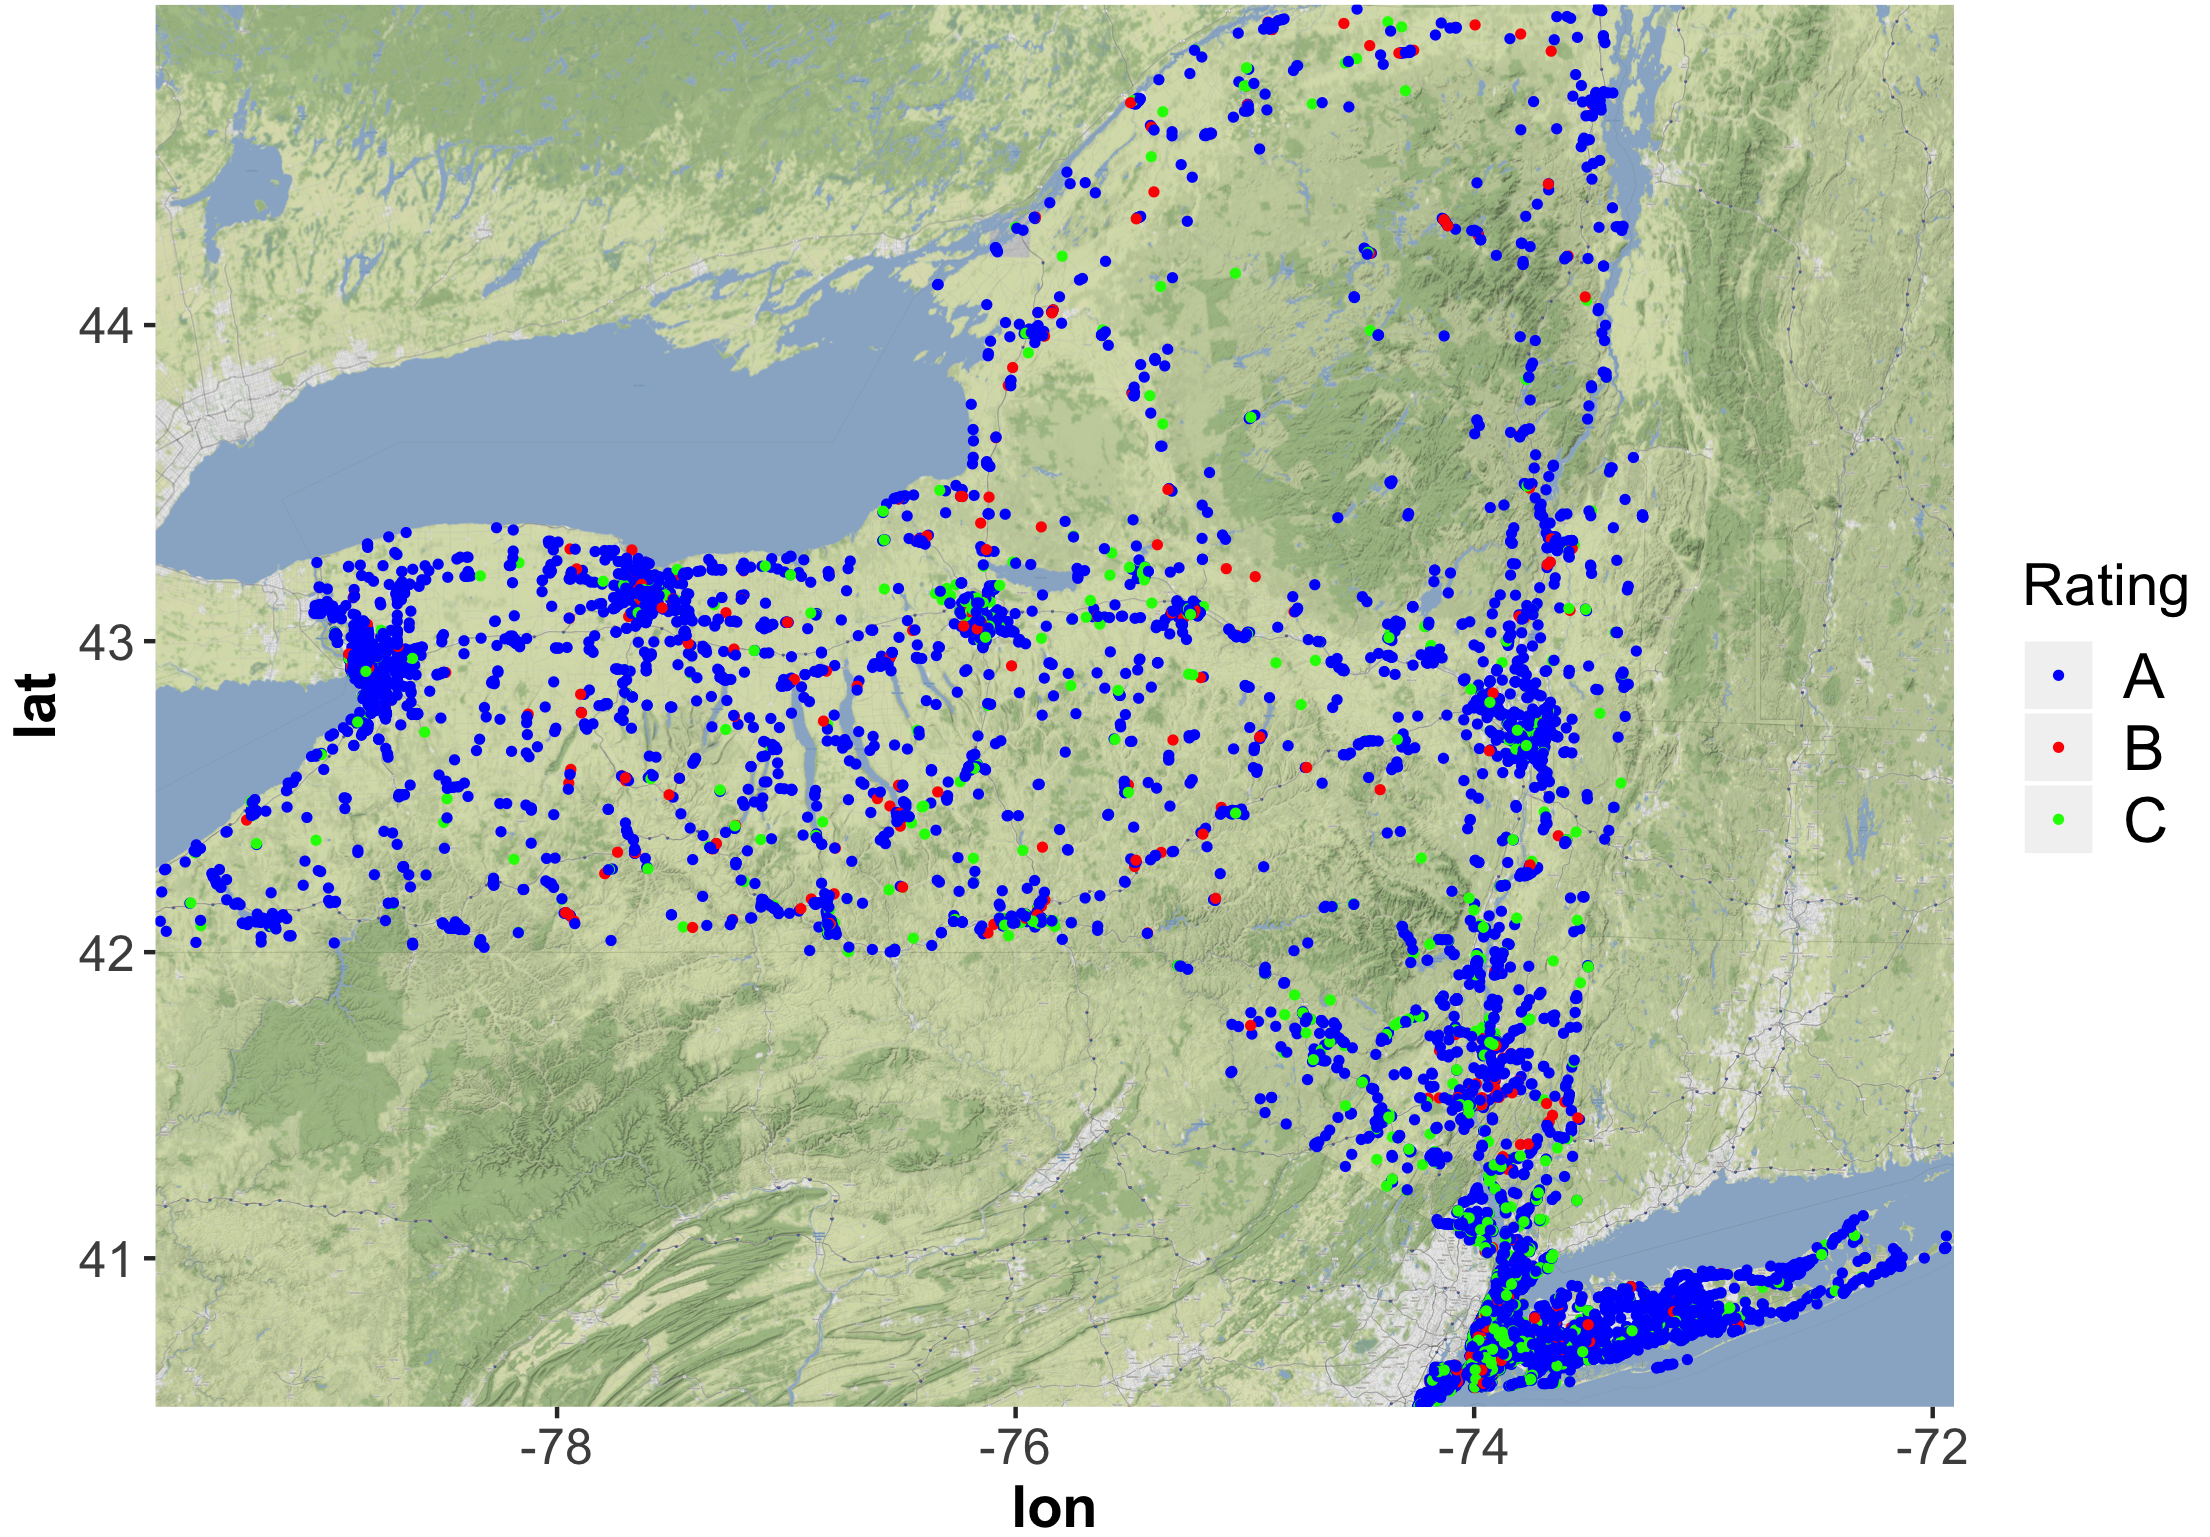
\includegraphics[width=0.5\textwidth]{Plots/Plot1_Map.png}
     }
     \hfill
     \subfloat[New York City]{%
       \includegraphics[width=0.5\textwidth]{Plots/Plot2_Map.png}
     }
\end{figure}
With complete spatial information, we now compute the two variables "shops density in 1km radius" as well as "rating of the closest neighbor". To get the distances of coordinates in meters, we apply the Haversine Formula\footnote{The Haversine Formula has its roots in spherical trigonometry and calculates the geodesic distance -- the shortest path between two points on a curved surface of a sphere, like the Earth. It needs to be mentioned that Haversine Formula does not take into account changes in altitude. However, it provides sufficient accuracy for the scope of this project.}
\begin{equation} a = \sin^{2}(\frac{\Delta\alpha}{2}) + \cos(\alpha_{1})\cos(\alpha_{2})\sin^{2}(\frac{\Delta\lambda}{2})  \end{equation}
\begin{equation} d = R \left( 2 \atantwo (\sqrt{a}, \sqrt{1-a} )  \right) \end{equation}
where $\alpha_{i}$ are latitudes, $\lambda_{i}$ are longitudes, $R$ is the earth's radius ($6371\times10^{3}m$).

\section{Subway Data}

In a next step, we amend our New York City inspection data with location information of subway stations. We use again \href{https://data.ny.gov/Transportation/NYC-Transit-Subway-Entrance-And-Exit-Data/i9wp-a4ja}{an official dataset provided by the State of New York}. The dataset contains the location of every subway entrance and its corresponding station. We are only interested in the station. Therefore, we remove all duplicates of stations with multiple entrances and then use again the Haversine Formula to find the distance of the closest station to every shop.


\Chapter{Conclusion}
--> Wrong predictors

\end{document}